\section{Faktoren des Klimasystems}
% Abbildung, die nach und nach wächst, mit den erklärten Teilbereichen

% vgl IPCC AR5 climate feedbacks, AR4 chapter 1 basics: carbon cycle

\begin{frame}
  \frametitle{Faktoren des Klimasystems}
  \begin{columns}
  	\column{0.4\linewidth}
	Atmosphäre \\
	Hydrosphäre = Ozeane und Wasserkreislauf \\
	Kryosphäre = Eismassen \\
	Biospähre = Tiere und Pflanzen \\
	Pedosphäre = Boden \\
	Lithosphäre = Gestein 
	\column{0.6\linewidth}
	\begin{figure}
	 	\centering
	 	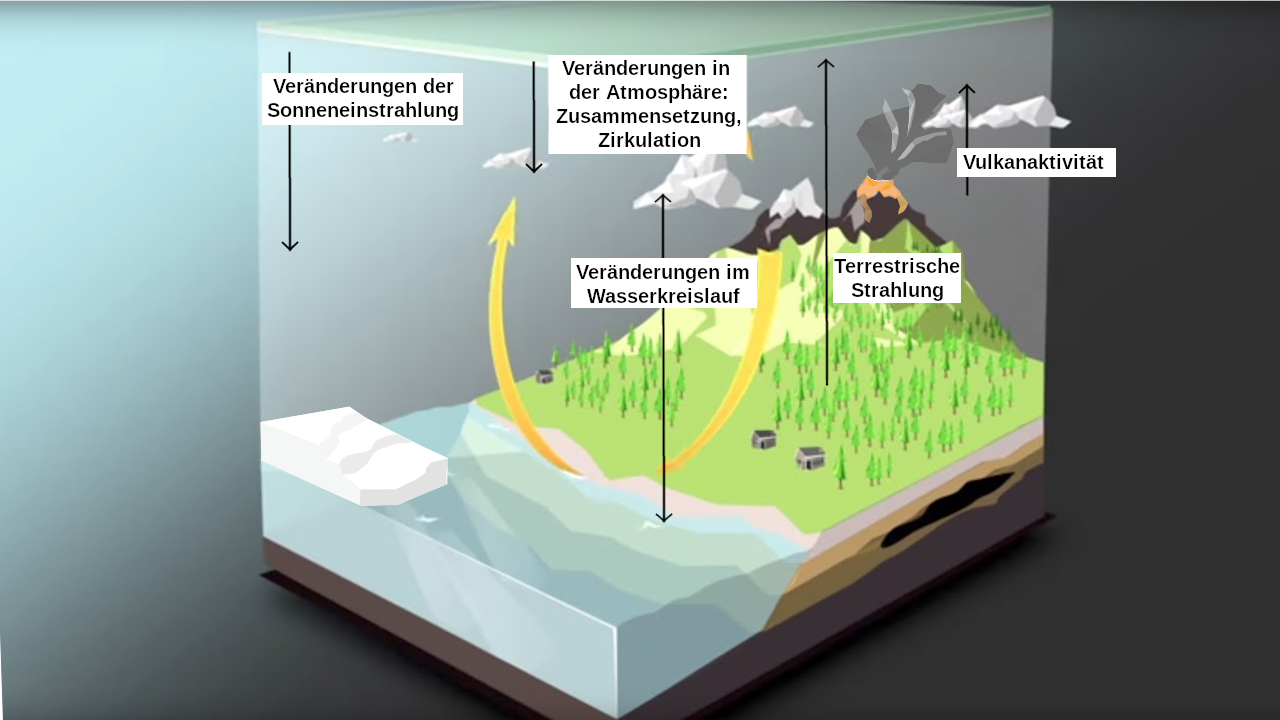
\includegraphics[width=0.8\linewidth]{bilder/WMO_Cycles_factors_general.png}
	 	\caption{Schematische Abbildung des Klimasystems, Quelle: IPCC 2007, Kapitel 1 und WMO-Video: The Carbon Cycle} % Anmerkungen hinzugefügt nach 
	\end{figure}
	%TODO: Evtl Bezeichnungen in Bild einfügen anstatt separat auflisten
	\end{columns}

\end{frame}


\begin{frame}
	\frametitle{Hydrosphäre - Wassermassen}
	\begin{figure}
		\centering
		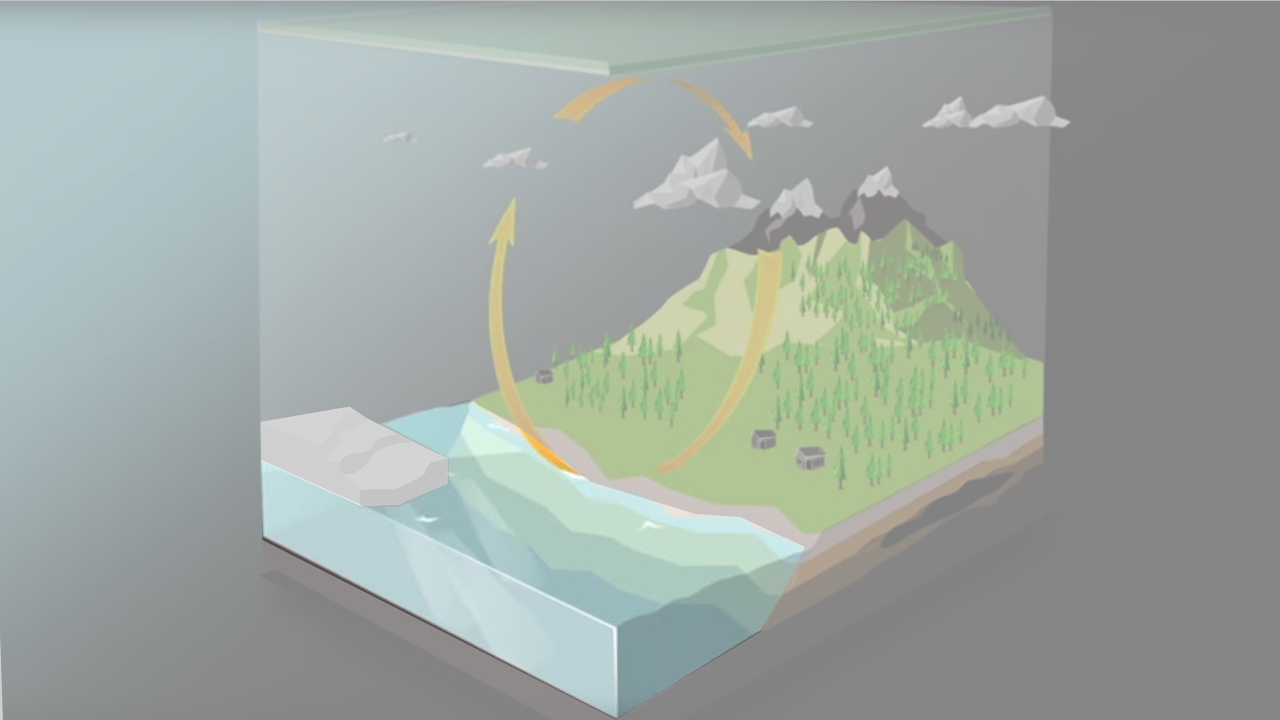
\includegraphics{bilder/WMO_Cycles_water.png}
		\caption{}
	\end{figure}
\end{frame}


\begin{frame}
	\frametitle{Hydrosphäre - Wassermassen}
	\begin{itemize}
		% Aufteilung von https://www.lenntech.de/faq-wasser-menge.htm, aber auch Wetzel, Robert G. 1983 in "Periphyton of freshwater ecosystems"
		\item Ozeane - Salzwasser ca. 97\,\%
		\item Flüsse und Seen - Süßwasser $<$ 1\,\%
		\item Eismassen ca. 2\,\% % zu den Eismassen gibt es einen extra Abschnitt
	\end{itemize}
\end{frame}


\begin{frame}
	\frametitle{Strahlungseigenschaft des Wassers} % M.Latif Klimawandel und Klimadynamik S. 23
	\begin{itemize}
		\item Wasser ist ein Dipol-Molekül \textcolor{blue}{$H_2O$}
		\begin{itemize}			
			\item<2->[$\rightarrow$] Kann viel Wärme aufnehmen bevor es verdampft $\rightarrow$ "Trägheit"
			\item<2->[$\rightarrow$] Kann wirksam Infrarotstrahlung absorbieren
		\end{itemize}
		
		%Allgemein liegt die größte Dichte des Wassers bei 4 Grad
		\item<3-> Größte Dichte des Wassermoleküls bei \SI{4}{\degreeCelsius}
		\begin{itemize}
			\item<4->[$\rightarrow$] Eis schwimmt auf Wasser
		\end{itemize}		
		% Im besonderen Fall des Salzwassers liegt die größte Dichte jedoch bei -3.8 Grad
		\item<5->Größte Dichte des Wassermoleküls in Salzwasser \SI{-3,8}{\degreeCelsius}
		\begin{itemize}
			\item<6->[$\rightarrow$] Bis zur Eisbildung sinkt kaltes Wasser in die tieferen Schichten des Ozeans
			\item<6-> [$\rightarrow$] Wärmeres, weniger dichtes Wasser steigt auf
			\item<6-> [] \textbf{\textcolor{blue}{Konvektion}} in den Polarregionen 
			\item<6-> [$\rightarrow$] Kohlenstoffsenken
		\end{itemize}
	\end{itemize}

% TODO: evtl. Abbildung der Konvektion: Abgabe von Wärme bei Aufnahme von atmosphärischen Gasen, die dann in die Tiefsee gelangen und dort gespeichert werden

%TODO: Erklärung von Senken
\end{frame}

\begin{frame}
	\frametitle{Wasserdynamik} %M. Latif Klimawandel und Klimadynamik S.24
	\begin{block}{Windgetriebene Zirkulation: } % eher horizontal
		Oberflächenströmung der Ozeane durch Reibung, Erdrotation (Corioliskraft) und Form der Meeresbecken 
	\end{block}
	\begin{block}{Dichtegetriebene Zirkulation: }  % eher vertikal
		Erwärmung, Abkühlung, und Änderung des Salzgehaltes (durch Eisbildung, Verdunstung oder Niederschlag) haben Einfluss auf die Dichte des Wassers, wodurch die Wassermassen zirkulieren
	\end{block}
	
	% Teil-Abbildung hier einfügen mit Ozean, Flüssen, Sonne, Verdunstung, Wolken und Niederschlag
\end{frame}


\begin{frame}
	\frametitle{Wirkung des Wassers auf das Klima}
	\begin{itemize}
	\item Ca. 70\,\% der Erdoberfläche ist mit Wasser bedeckt
	\item [$\rightarrow$] Die \textit{Trägheit} des Wassers ist ein entscheidender Faktor für die Trägheit des Klimas und der Klimaänderungen % M.Latif Klimawandel und Klimadynamik S. 23
	\item Kohlenstoffsenken in der Tiefsee können durch erwärmen der Ozeane *irgendwann* freigesetzt werden
	\item[$\rightarrow$] massiver Anstieg des atmosphärischen $CO_2 \rightarrow$ Verstärkung des Treibhauseffekts
	\item Positive Verstärkung von $CO_2$ und Wasserdampf: eine wärmere Atmosphäre kann mehr ($CO_2$ und) Wasserdampf aufnehmen
	\end{itemize}
\end{frame}

\begin{frame}
	\frametitle{Trägheit des Klimas}
	Die Trägheit des Klimas zeichnet sich dadurch aus, dass Feedbacks verzögert zu einem klimawirksamen Ereignis auftreten. Das heißt, die einzelnen Komponenten des Klimasystems benötigen eine gewisse Zeit sich in den veränderten Bedingungen des Systems zu stabilisieren
	
	
	\begin{figure}
		\centering
		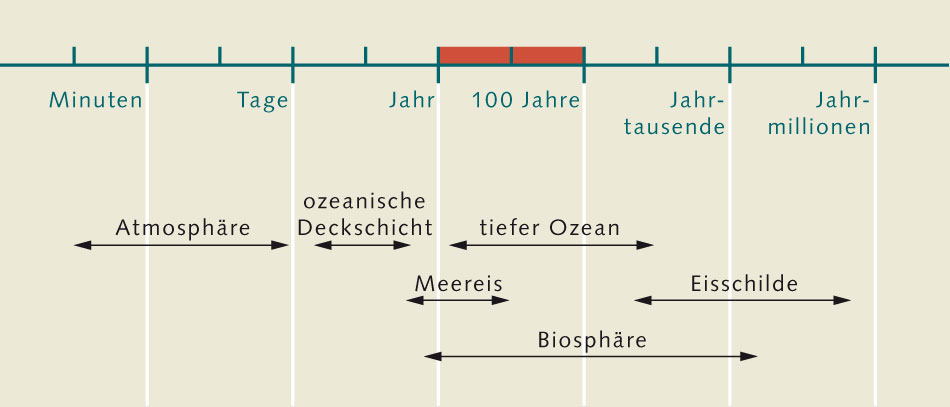
\includegraphics[width=0.8\linewidth]{bilder/zeitskala-klimasystem_world_ocean_review.jpg}
		\caption{Zeitskalen im Klimasystem, Quelle: maribus nach Meinecke und Latif, 1995}
	\end{figure}
	
	Besonders die Ozeane und Eisschilde benötigen demnach eine sehr lange Zeit, um sich geänderten klimatischen Bedingungen anzupassen.
\end{frame}

\begin{frame}
	\frametitle{Kryosphäre - Eismassen}
	
	\begin{figure}
		\centering
		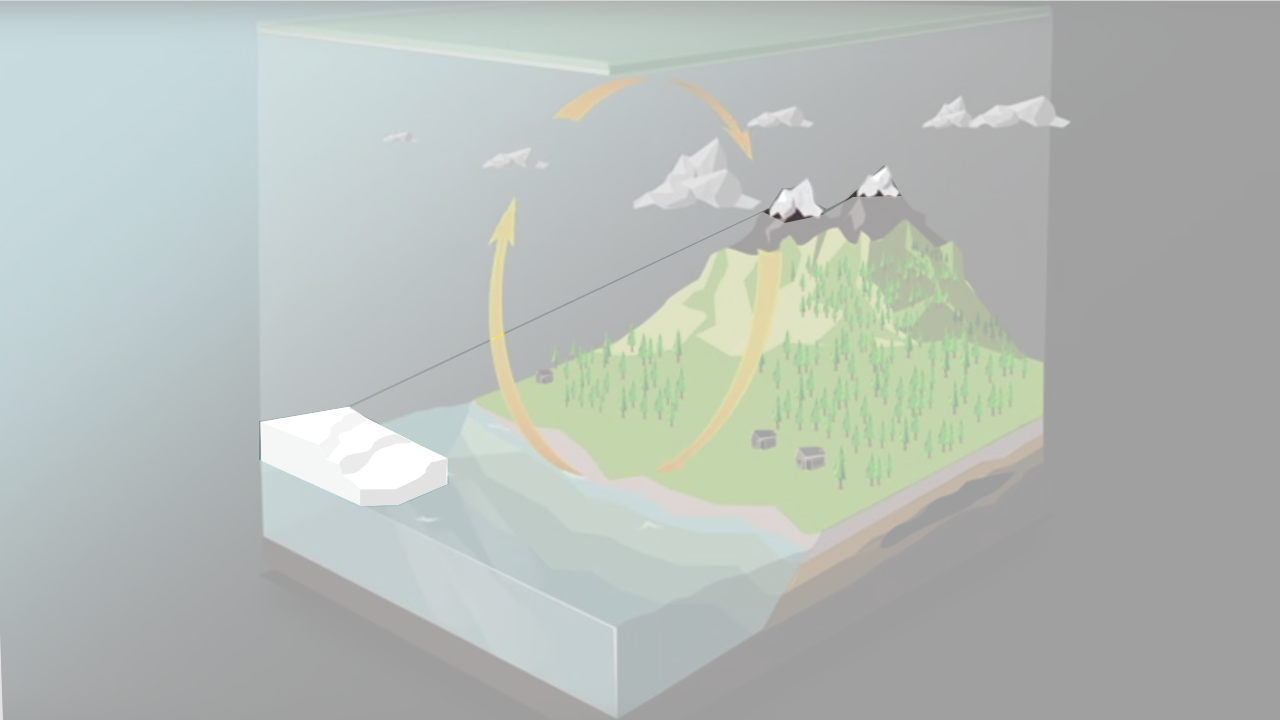
\includegraphics{bilder/WMO_Cycles_ice.png}
		\caption{Kryosphäre umfasst alle Formen und Schnee und Eis}
	\end{figure}
\end{frame}

\begin{frame}
	\frametitle{Kryosphäre - Eismassen} % Eismassen der Erde
	\begin{itemize}
		\item ca. 2\,\% des Wassers ist in fester Form in Gletschern und an den Polkappen dauerhaft gebunden.
		\item Eis reflektiert die ankommende Sonnenstrahlung zu großen Teilen
		$\rightarrow$ \textbf{\textcolor{blue}{Albedo-Effekt}}\\
		
		\item Je weniger Eismassen, desto weniger Strahlung wird reflektiert und bleibt in der Atmosphäre $\rightarrow$ Verstärkung des Treibhauseffekts
		
		\item Durch Rußablagerungen auf den Eismassen wird mehr Sonnenstrahlung absorbiert 
		\item [$\rightarrow$] Schmelzen des Eis und Verringerung des Albedo-Effekts % (Nature Geoscience, 2014; doi: 10.1038/ngeo2180) 
	\end{itemize}
	
\end{frame}

\begin{frame}
	\frametitle{Permafrost}
	%TODO evtl. Exkurs zu Permafrost an dieser Stelle, da er unter die Kryosphäre fällt
\end{frame}

\begin{frame}
	\frametitle{Interaktion Hydrosphäre, Kryosphäre und Atmosphäre}
	\begin{figure}
		\centering
		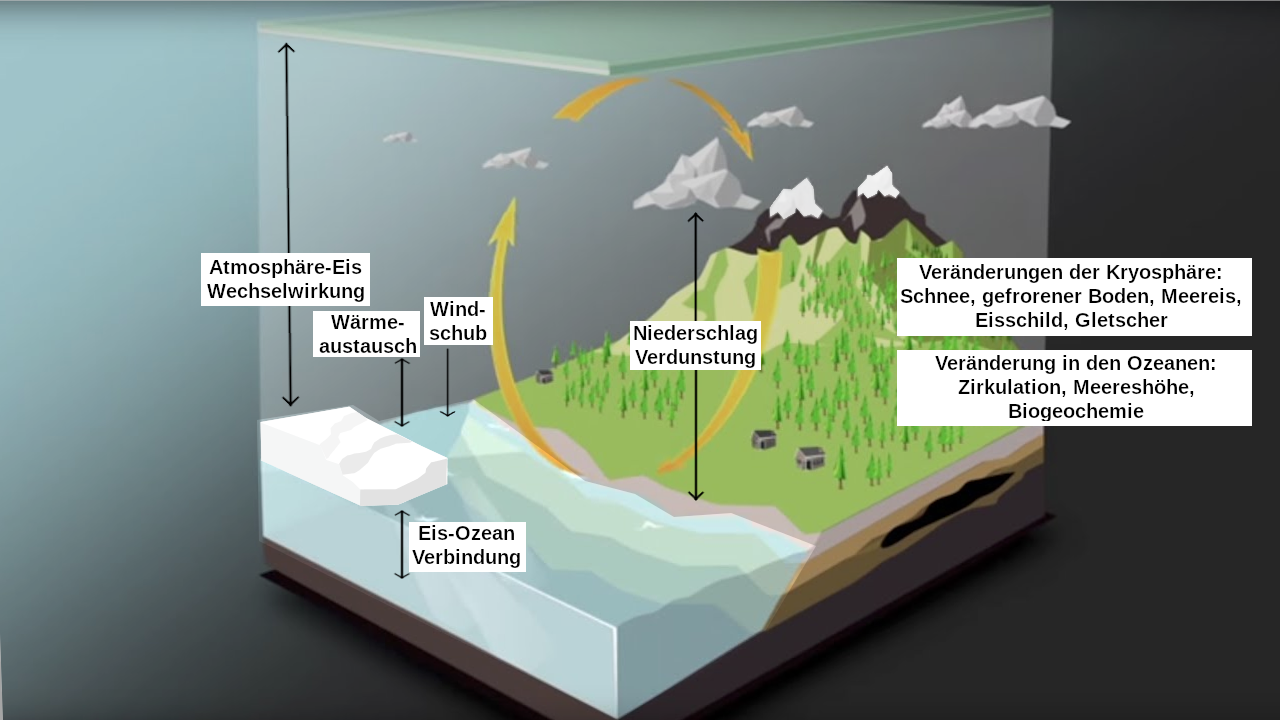
\includegraphics{bilder/WMO_Cycles_factors_waterAndIce.png}
		\caption{Interaktion Hydrosphäre, Kryosphäre und Atmosphäre}
	\end{figure}
\end{frame}

\begin{frame}
	\frametitle{Vegetation und Böden}
	
	\begin{figure}
		\centering
		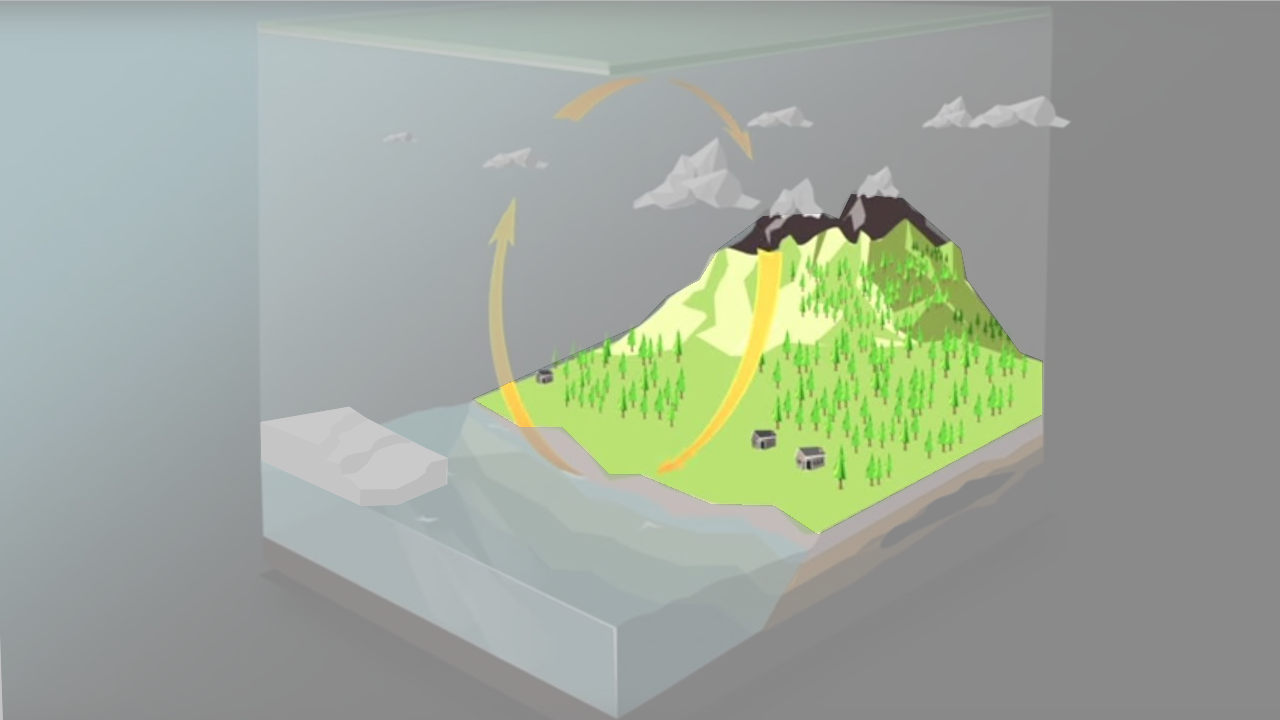
\includegraphics{bilder/WMO_Cycles_land.png}
		\caption{}
	\end{figure}
\end{frame}

\begin{frame}
	\frametitle{Vegetation}
		%TODO -z.B. in  M.Latif: Kap 1.3.4
\end{frame}


\begin{frame}
	\frametitle{Interaktion Vegetation und Atmosphäre}
	
		\begin{figure}
		\centering
		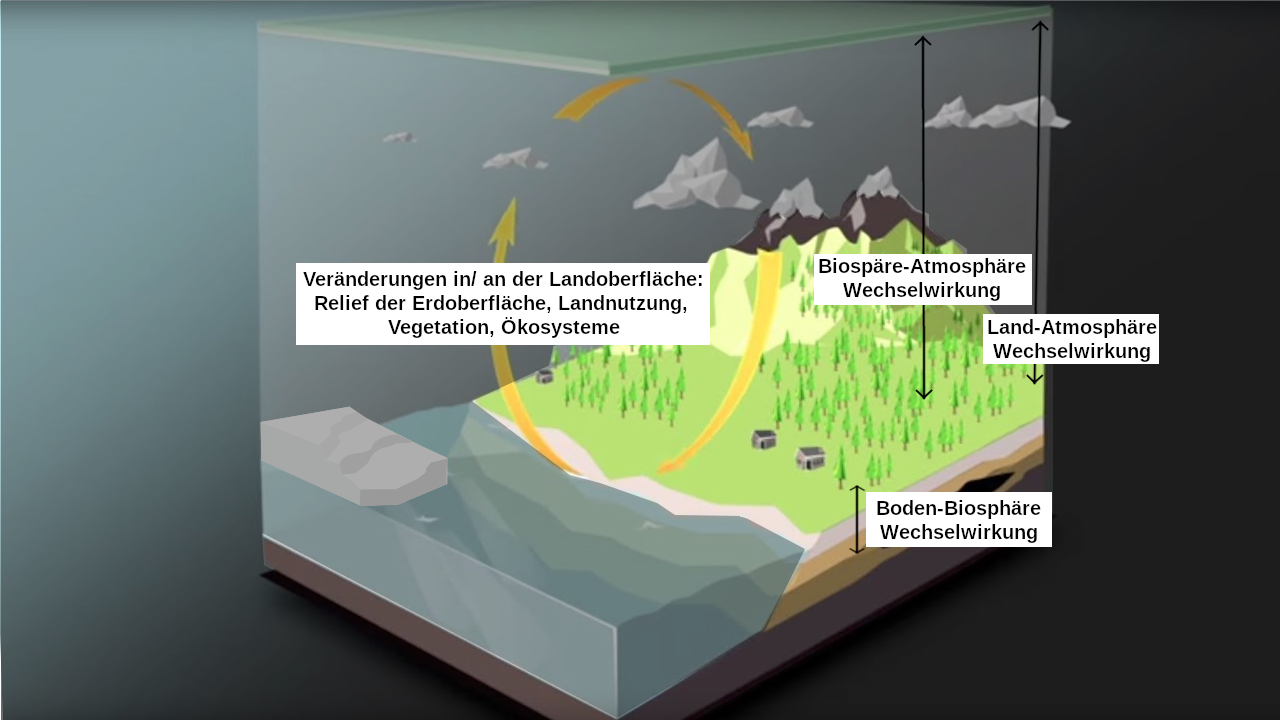
\includegraphics{bilder/WMO_Cycles_factors_landAndGround.png}
		\caption{Interaktion der Biosphäre und Atmosphäre}
	\end{figure}

\end{frame}



\begin{frame}
	\frametitle{Das Klimasystem - Zusammenfassung}
	% Abbildung mit allen zuvor erklärten Elementen
	
	\begin{figure}
		\centering
		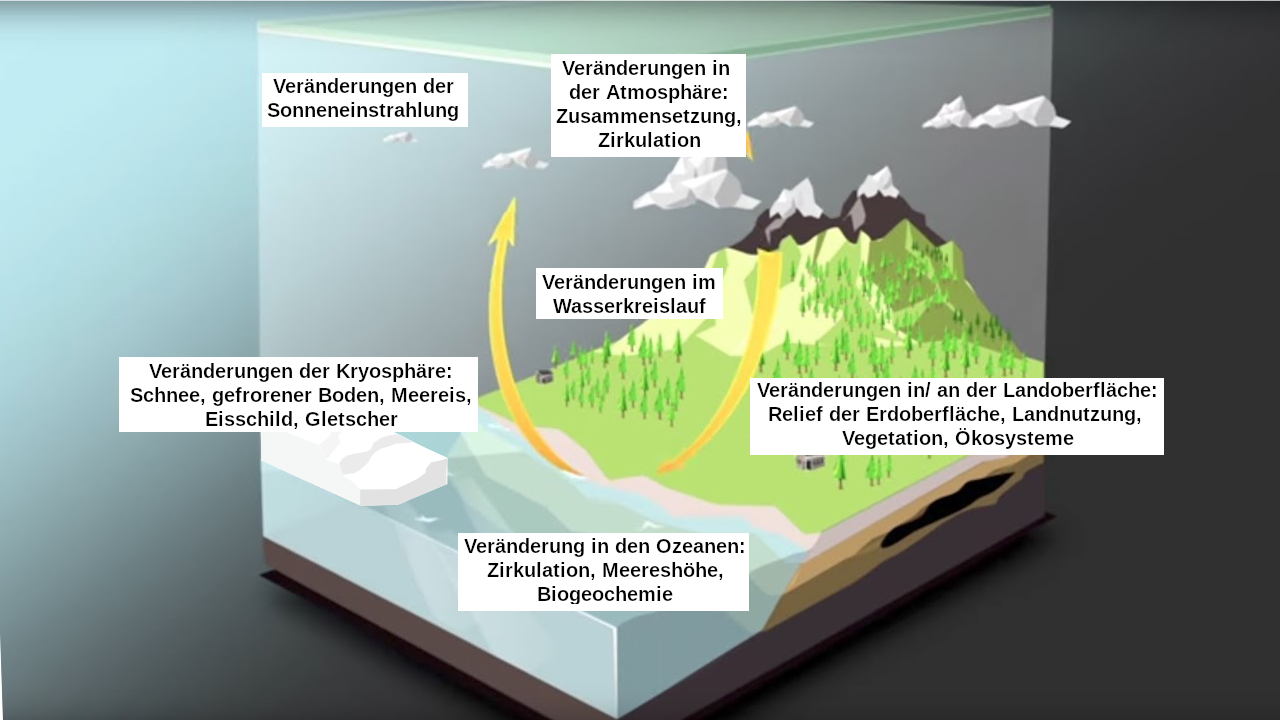
\includegraphics{bilder/WMO_Cycles_overview.png}
		\caption{Abbildung des Klimasystems mit allen zuvor erklärten Elementen}
	\end{figure}
\end{frame}


\begin{frame}
	\frametitle{Kohlenstoffkreislauf}
	
	% nach der Vegetation und Lebewesen
	% --> mit Fokus Fabriken und Ausstoß von CO2
	
	\begin{figure}
		\begin{columns}
			\column{0.6\linewidth}
		\centering
		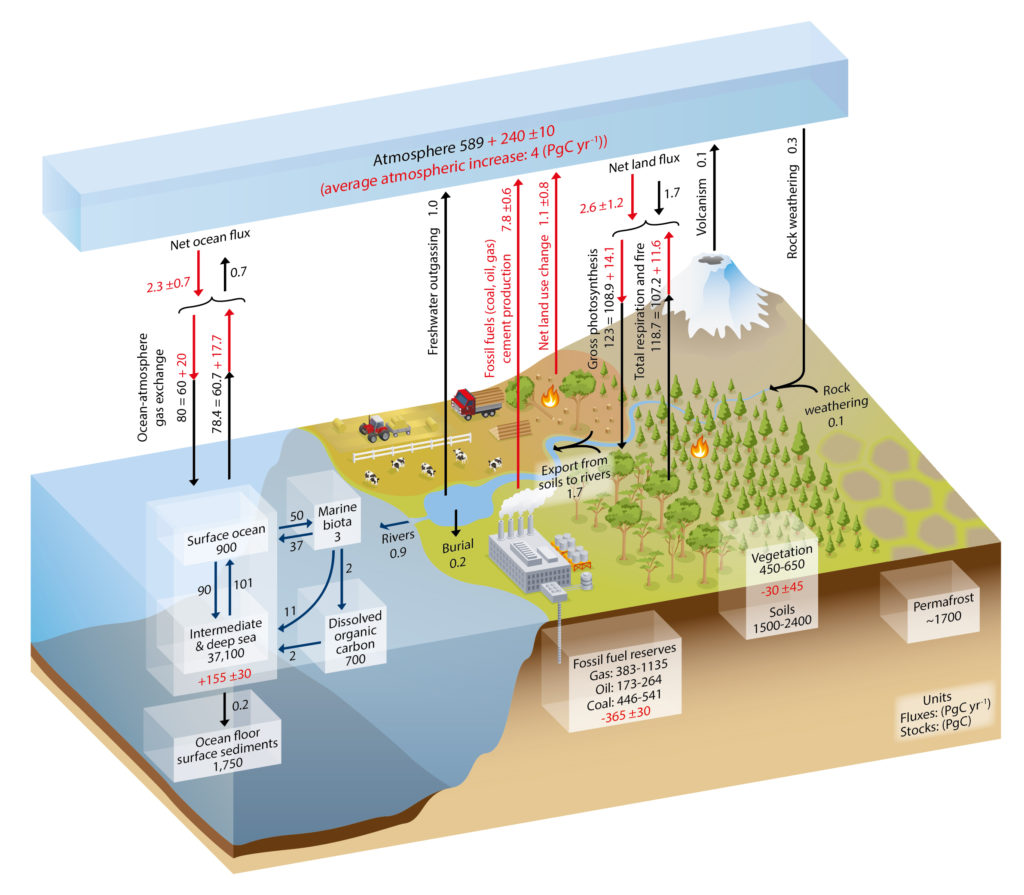
\includegraphics[width=0.9\linewidth]{bilder/IPCC_Cycles_carbon.jpg}
		\column{0.4\linewidth}
		\caption{Vereinfachte Abbildung zum Kohlenstoffkreislauf, Quelle: IPCC 2014, Kapitel 6}
		\end{columns}
	\end{figure}
	
	\color{red}\textbf{rot}\color{black}: durch Menschen verursachte mittlere jährliche $CO_2$ Flüsse im Zeitraum 2000-2009 \\% es ist anzunehmen, dass die Werte heute nochmal höher sind als die angegebenen
	\textbf{schwarz}: vermutete natürliche $CO_2$ Flüsse vor der Industrialisierung (vor 1750)
	% Wichtig hierbei ist vorallem das Fazit, dass der CO2 Gehalt der Atmosphäre sich seit der Industrialisierung beinahe verdoppelt hat!
\end{frame}


% Aber nicht nur der CO2 Gehalt der Atmosphäre hat sich erhöht, sondern auch der von Methan und Lachgas:
\begin{frame}
	\frametitle{Atmosphärisches Methan und Lachgas}
	
	% nach der Vegetation und Lebewesen
	% --> mit Fokus Fabriken und Ausstoß von CO2
	
	\begin{figure}
		\begin{columns}
			\column{0.5\linewidth}
				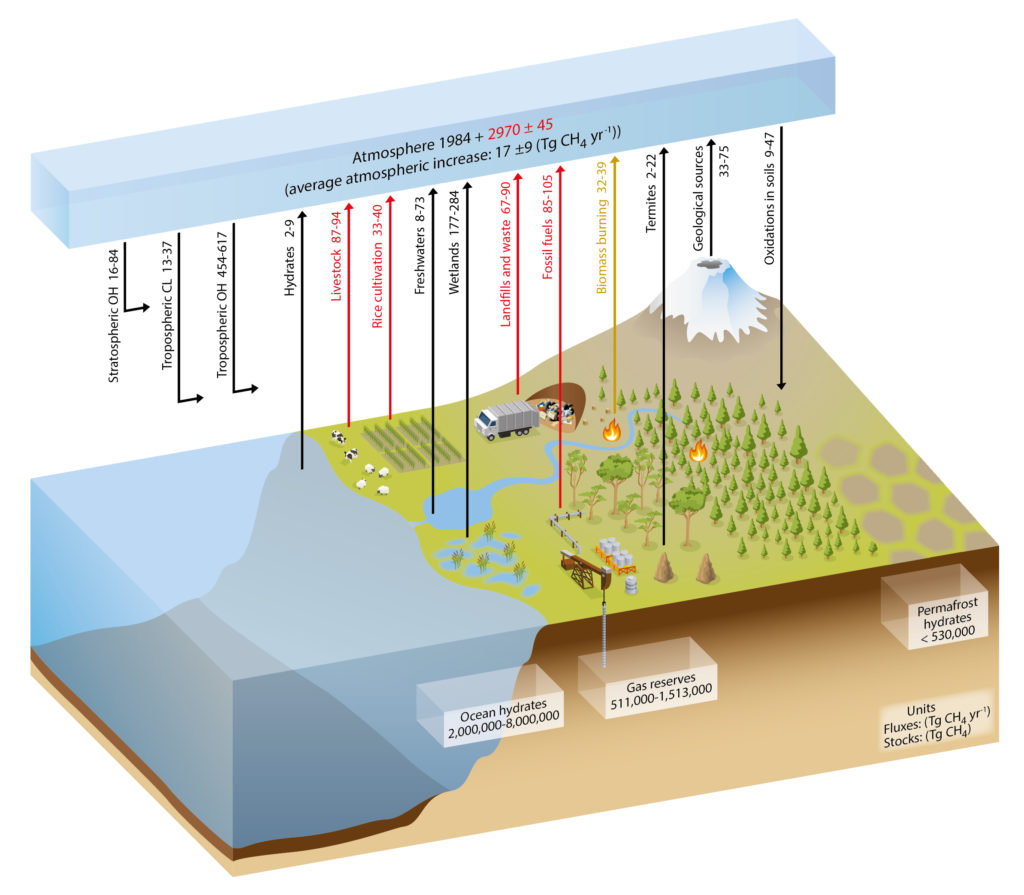
\includegraphics[width=\linewidth]{bilder/IPCC_Cycles_methane.jpg}
			
			\column{0.5\linewidth}
				\centering
				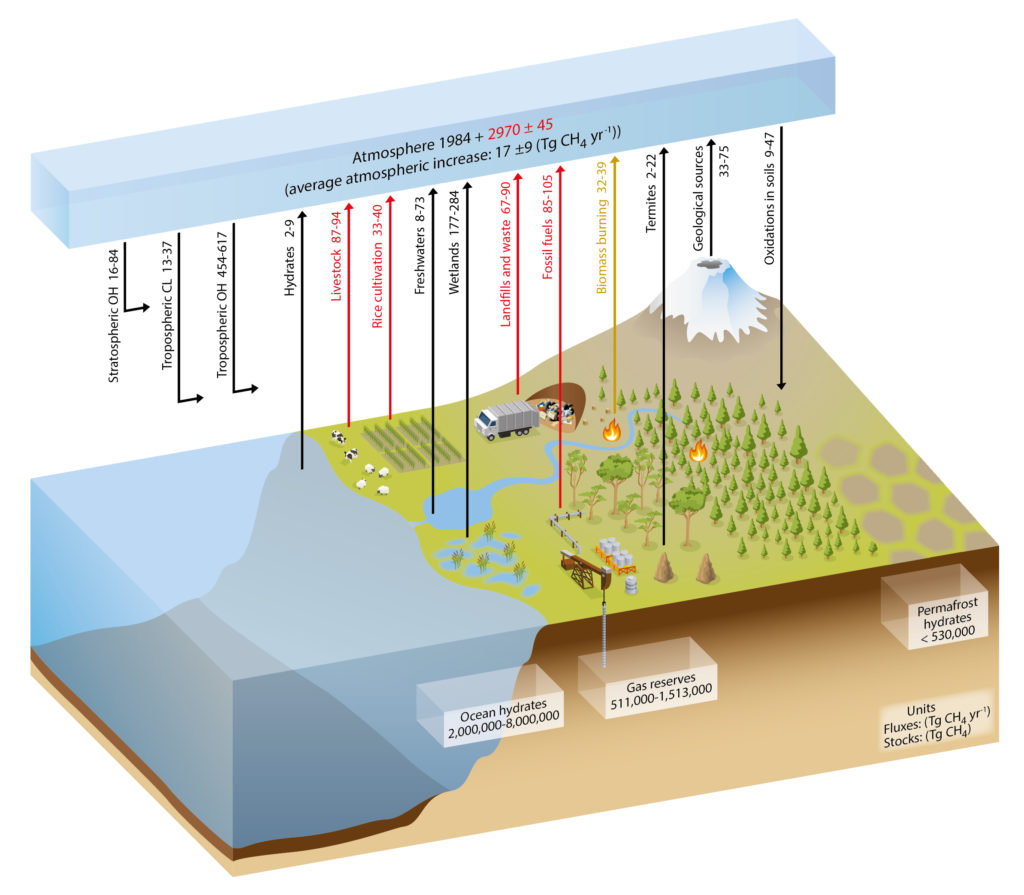
\includegraphics[width=\linewidth]{bilder/IPCC_Cycles_methane.jpg}
		\end{columns}
		\caption{Vereinfachte Abbildung zum Methan und Lachgaskreislauf, Quelle IPCC 2014, Kapitel 6}
	\end{figure}

	\vspace{-1cm}
	Der Gehalt an Methan in der Atmosphäre hat sich um 250 \,\% erhöht, der Gehalt von Lachgas um etwa 20 \,\%

\end{frame}


%Folgende Folie(n) eher nicht einbringen?

%\begin{frame}
%	\frametitle{Atmosphäre}
%	
%\end{frame}

